\documentclass[onecolumn, draftclsnofoot,10pt, compsoc]{IEEEtran}
\usepackage{graphicx}
\usepackage{url}
\usepackage{setspace}
\usepackage{array}
\usepackage{tabu}
\usepackage{listings}
\usepackage{geometry}
\geometry{textheight=9.5in, textwidth=7in}
\graphicspath{ {images/} }
% 1. Fill in these details
\def \CapstoneTeamName{		Deep Learning on Embedded Platform}
\def \CapstoneTeamNumber{		14}
\def \GroupMemberOne{			Christopher Johnson}
\def \GroupMemberTwo{			Gabe Morey}
\def \GroupMemberThree{			Luay Alshawi}
\def \CapstoneProjectName{		AI Gaming}
\def \CapstoneSponsorCompany{	NVIDIA}
\def \CapstoneSponsorPerson{		Mark Ebersole}

\def \DocType{	%Problem Statement
				%Requirements Document
				%Technology Review
				%Design Document
				Progress Report
				}

\newcommand{\NameSigPair}[1]{\par
\makebox[2.75in][r]{#1} \hfil 	\makebox[3.25in]{\makebox[2.25in]{\hrulefill} \hfill		\makebox[.75in]{\hrulefill}}
\par\vspace{-12pt} \textit{\tiny\noindent
\makebox[2.75in]{} \hfil		\makebox[3.25in]{\makebox[2.25in][r]{Signature} \hfill	\makebox[.75in][r]{Date}}}}

\begin{document}
\begin{titlepage}
    \pagenumbering{gobble}
    \begin{singlespace}
    	% 
\includegraphics[height=4cm]{coe_v_spot1}
        \hfill
        % 4. If you have a logo, use this includegraphics command to put it on the coversheet.
        %\includegraphics[height=4cm]{CompanyLogo}
        \par\vspace{.2in}
        \centering
        \scshape{
            \huge CS Capstone \DocType \par
            {\large\today}\par
            \vspace{.5in}
            \textbf{\Huge\CapstoneProjectName}\par
			\vfill
            {\large Prepared for}\par
            \Huge \CapstoneSponsorCompany\par
            \vspace{5pt}
            {\Large\NameSigPair{\CapstoneSponsorPerson}\par}
            {\large Prepared by }\par
            Group\CapstoneTeamNumber\par
            % 5. comment out the line below this one if you do not wish to name your team
            \CapstoneTeamName\par
            \vspace{5pt}
			{\Large
                \NameSigPair{\GroupMemberOne}\par
                \NameSigPair{\GroupMemberTwo}\par
                \NameSigPair{\GroupMemberThree}\par
            }
            \vspace{20pt}
        }
        \begin{abstract}
        In this document we describe what we have done with our project to create a deep learning program that can learn to play the game Galaga.
	This project will be used as a training tool for NVIDIA's Deep Learning Institute.
	We briefly describe the purpose of the project, the progress we made, and the problems we faced throughout development.
	We also set forward some goals and plans to finish out the year and hand off the project to NVIDIA.

        \end{abstract}
    \end{singlespace}
\end{titlepage}

\newpage
\pagenumbering{arabic}
\tableofcontents

\section{Project Purpose}
The main goal of our project is to create a neural net that can learn to play the game Galaga.
The neural network must run on NVIDIA's Jetson developer kit, as this was one of the requirements for the project.
This project will be used by trainers and students in the field of deep learning.
NVIDIA's Deep Learning Institute will take the work that we do and use it to create a learning course.
It must be possible to recreate this project, or it will not make a good learning tool.
As such, our documentation had to be detailed enough to give readers a clear understanding of how we made the system.

\section{Current Progress}
Throughout the first term we laid out all the ground work for out project.
We've created documentation for our project requirements, our decisions for the technology that we want to use, and how we will be using that technology in our project.
These documents have been given to our client who has signed and returned them to ensure that everything can be smoothly recreated and used in an educational setting.
\newline\newline
Over winter break we began implementation.
The project at present has the following components: a neural network still in the stages of training to properly identify in game objects, a set of python scripts implementing port communication protocol to allow the neural network to converse with the system hosting the game, and a hardware setup with camera to allow the Jetson to see what's happening on the other computer.
Though there are many bugs to iron out, the system can generate actions based on the situation of the player, and commands can be given to the game from the neural network.
Moving forward the main goals are increasing the speed of command, the accuracy of gameplay, and ironing out bugs.

\section{Problems and Solutions}
We ran into several problems throughout the first term.
One problem we had was our busy schedules.
It was difficult to find times to meet up and work on projects.
We had to schedule our weekly TA meeting on Fridays which wasn't ideal.
Our TA is planning on scheduling all his meetings on Monday which might help for Winter term.
We're also handling this problem by improving our lines of communication with each other.
By staying in touch regularly and planning ahead, we have mitigated a lot of the scheduling issues that have plagued this term.
\newline\newline
Another problem we had was getting our documents signed.
Our client was very busy throughout the term and it took a while to to get responses from him.
All of our assignments were either turned in late or without a signature.
He said that his schedule should soon be clearing up and he won't have to travel as much so it shouldn't be as bad next term.
Just in case our client remains difficult to contact we planned to ask him about more methods of contact as well as maybe finding other people at the company who can weigh in when he's unavilable.
\newline\newline
Another problem arose in this project due to the vagueness of the initial project.
Initially, we had no solid idea what our project was going to be, other than that it had to involve a neural network.
Issues contacting our client compounded this issue as we needed information about what kinds of projects would be considered suitble for the task at hand.
Eventually we were able to establish solid enough contact to determine our actual task.
\newline\newline
The final issue first term arose from the difficulty of actually understanding neural networks.
Learning about neural networks required much more research than we initially assumed, and the field is incredibly complex.
In order to better understand what was going on, we had to try and cram tons of research into a very small period.
This met with middling success and we still weren't fully confident in our design.
We did, however, have a solution in mind.
We reached out to our client and made contact with an engineer at NVIDIA.
We also took advantage of the increased free time during winter break to more thoroughly study our subject and prepare the initial system.
\newline\newline
The second term started off with a long winter break, during which major breakthroughs and problems were discovered.
Perhaps the biggest thing to come out of winter break was a new understanding what exactly we had to do to get our neural network functioning.
By the end of the break we had a much more solid plan for what we were going to accomplish.
However, our initial approach to the network required some custom implementation that we weren't sure how to do yet.
We didn't know how to get the neural net telling the game how to play.
To solve this, we spoke with our client and he connected us with an engineer at NVIDIA who had more experience with neural networks.
With his help, we came to the decision of implementing a single decision layer into the neural net that would take the output of the image processing layers and produce an output in the form of a game command.
\newline\newline
The next big problem we needed to approach was the setup we need to use to get the setup correct for playing the game.
Because we need to have the Jetson run the neural network, we've been gathering parts to allow us to put Galaga on a PC seperate from the jetson for playing.
We've purchased a camera to watch the screen of the other PC and send that back as input.
At the moment reflectivity is hampering this process, so we are working on getting a screen with as little reflectiveness as possible.
Another major part of this setup was getting a program setup that could relay the commands from the neural net to the game.
To solve this, we set up a basic communication server setup through python, which waits for commands and then simulates the keypresses ordered through a Windows api.
\newline\newline
The major issue that hung over our heads heading into the end of winter term was the speed the neural network.
On a normal PC, our system actually ran decently, but the Jetson is considerably slower.
With average processing speed between 3 and 9 fps (frames per second) when implemented on the Jetson, our network was simply too slow to play a 60 fps game right now.
We tested ways around this limitation and eventually improved the speed.
\newline\newline
The biggest improvement to the project since the middle of winter term was the frame rate.
We now get around 12-15 frames processed per second with the neural network.
This is possible because of optimizations we found for the Jetson that help divert resources to running a neural network.
We set our sights on improving the decision layer code, as well as getting the neural network trained further.
\newline\newline
In order to get ready for Expo this term, we started with a few goals.
Goal number one was to get our neural network trained better.
Goal number two was to improve the decision layer logic for the network.
Our final goal was to buff up the frame rate of the neural network response.
Along the way we also had to finish the poster for expo and prepare to present.
\newline\newline
Getting the neural network trained was a matter of continuing to do what he'd done for a while now.
We needed to gather more images and annotate them for the training process.
Getting more images was a central part of getting the project ready for expo.
We've managed to build up a good image base with over one hundred annotations.
After the latest training run, our detection results have proved better than ever before.
\newline\newline
When it came to the decision layer logic, we tried quite a few methods.
Our initial logic only allowed the network to move away from incoming enemies or shoot them.
After a bit more refinement, we tried a version where the system was allowed to shoot, then move in one command.
This second version had some better performance and its results were used on our expo poster due to the time in term.
Afterwards, we arrived at what is now the final and best version of the decision layer.
This version moves much more often and can prepare to fire when it sees no enemies.
This version also tends to shoot whenever it moves.
This combination helps it find enemy targets as well as shoot reflexively at oncoming enemies.
With this version, we've come to meet our goal of beating the first level of Galaga 90\% of the time.
\newline\newline
The framerate is the goal we've consistently had the most trouble meeting.
While framerate was not a part of our requirements, we wanted to have a reasonable play speed to make the network more exciting.
However, we've never gotten much more than 15 FPS out of the Jetson. 
Pushing the game speed up higher results in the Jetson responding too slow to perform well.
We tried using some optimization tools from NVIDIA, but they didn't properly support the SSD basis of our neural network or its custom layers.
We have signed up for the test of the new version, so we may yet be able to do something.
\newline\newline
One major issue we had to resolve this term was getting results for our poster.
When we first handed it off to our client, he liked what we had but wanted more concrete performance results from our neural network.
The week before the poster's due date became a challenging rush to optimize our system and get good results to put on the poster.
Ultimately, the poster turned out good and the results were usable. 
We do wish we could have had more time, however, as we've since achieved much better results, with a maximum score of 18230 and now being able to regularly beat level 1.
\newline\newline
Overall, we're very happy with the progress and outcome of this project, but we aren't done yet.
We continue to try and optimize it, and we have a lot of documentation to catch up on.
We're a far cry away from where we were at the start of the term, and we're better programmers for it.
That does mean, however, that most of the documentation written then does not match what our project has come to be.
While we do have some edits done from last term, we still have a lot to catch up on if we are to meet the requirements of the class.
It's also important that our documentation be excellent because NVIDIA needs to be able to recreate it as a Deep Learning Institute lab.
With that in mind, we have a lot of work cut out for us to finish this class.

\section{Retrospective}

\begin{center}
\begin{tabu} to 0.9\linewidth{ || X[l] | X[l] | X[l] || }
	\hline
	Positives & Deltas & Actions \\
	\hline\hline
	Decided on Galaga as main project & Need to improve system setup & Research more in depth how deep learning systems are constructed \\ \hline
	Found a way to work together despite scheduling problems & Need to carefully evaluate design of system to ensure robustness & Seek help from professors who research neural networks and ask our client if anyone at NVIDIA can give us some setup advice \\ \hline
	Finished all necessary documentation & Need to improve clarity and quality of documentation & Rewrite portions of documentation as our design improves to make sure our project's goals and design are clear \\ \hline
	Figured out a preliminary design with several tools we can use to make it work & Need to complete setup of the network to begin training & Begin working on neural network setup, particularly engaging phase 1, teaching the network how to recognize in game objects \\ \hline
	Researched more and figured out how to work our project & Need to fully finish the design & Will continue to update documentation as we figure more out about the specific challenges of the project \\ \hline
	Completed the alpha build of the project setup & Need to work out the kinks of our setup and continue training & Test the system intently and improve functionality \\ \hline
	Improved system speed & Need to increase FPS further & Will continue searching for optimizations \\ \hline
	Completed training to a satisfactory level & Could always use more training & We might try one more training run before expo \\ \hline
	Improved Decision Layer logic to consistently beat level 1 & Need to get documentation for project up to date & Will spend the rest of the term fixing and improving documents \\ \hline
\end{tabu}
\end{center}

\section{Week by week summary}

\subsection{Spring Week 1}
This week we had a lecture to prepare us for the coming months.
We have only training left to do before expo so this week we started creating annotations for the neural net's image detection.

\subsection{Spring Week 2}
This week I was able to get some annotations done and we found a group to discuss our poster with.
We're feeling pretty relaxed now that most of the work is done.
This week we were able to find a group to discuss our poster with for the extra credit.
Luay started working on improving the defense and attack algorithm.
Gabe decided to work on trying to run tensorRT on the Jetson TX1 and try to integrate it with SSD.
The plan for next week is to have work done on the decision layer algorithm and test it on the Jetson TX1 as well as home computer GPU.

\subsection{Spring Week 3}
Chris made more annotations.
We still have yet to meet with our team to discuss our poster.
We need to make a final draft soon.
We also have to get it to Mark as soon as possible since it will probably take him a while to get it signed.

\subsection{Spring Week 4}
This week we met up and figured out what we had left to do before the code freeze on May 1st.
We realized there was a lot on the requirements document that we still needed to update and we weren't sure if we could meet a lot of them by May 1st.
The neural net still isn't performing as well as it should be.
We fixed up our poster, got our group photo, and sent the poster to Mark and the professors.
We also asked the professors how much we needed to fix with the requirements document.

Luay was given a Jetson TX2 to test our project on.
The goal was to compare the performance between both the TX1 and TX2.
Due to the differences in GPU architecture on both boards the GPU performance of Caffe was slow.
This issue was solved by altering the makefile configuration.
The maximum performance with the TX1 that we could get was 10 FPS using our custom nerual network model.
On the other hand, Gabe was working on improving the decision algorithm on Jetson Tx1 and tensorRT.
There were some difficulties finding resources on integrating tensorRT.
Luay tried working on TensorRT as well as improving the decision layer.
Writing a tensorRT program unfortunately wouldn't work because tennsorRT does not support custom Caffe layers which was stated on the release note and was the complaint error when running the program.

By the end of the week the neural network played the game winning stage 1 90% of the time.
The highest score reached so far is 15520 which is a new record.
Also, the neural network was able to reach stage 4 of the game and this is the best result so far.
We are hoping to do a live demo during expo by having one Laptop that has the game and the Jetson TX1.
By using the camera on board we are going to save space and be able to do a live demo.

\subsection{Spring Week 5}
This week we got through the code freeze after making sure everything we used was in our repo.
We also finished our poster and submitted it for printing.
Luay recently was able to boost the performance of the neural net using screen capturing instead of video recording.
We will most likely continue working up until Expo on May 19th.
There are still two more lectures before then.

This week I continue working on installing OpenCV 3.2.0 to use the Jetson TX1 on board camera.
The onboard camera is better quality and capable of capturing full HD compare to the current USB camera which is only able to capture up to 720p.
The process of installing OpenCV 3.2.0 was painful because there was not enough disk space and had to spend the time to clean unnecessary files.
However, after cleaning the disk from unwanted files I was finally able to install OpenCV.
Although, the process of installing OpenCV from source code took more than an hour due to the low power nature of the Jetson TX1.
By using the onboard camera we might be able to do a live demo during the expo.
Finally, we are planning to email our client this week to give him updates on our current progress.

This week we submitted the poster and merged all our github repos for the the final code freeze.
Luay has been working on performance.
Meanwhile I've been turning my attention to documentation.
With Expo coming up and the final code done, we need to get our documentation on track for the end of the term.
I am starting with the requirements document, as the scope of the project has changed drastically since we wrote it.

\subsection{Spring Week 6}


\section{Code Sample}
\subsection{Python Script Plays the Game}
\begin{lstlisting}[language=Python,caption=Python script captures image and feed to nerual network to send a decision to the other computer.]
while True:
    flag, frame = cap.read() # Capture image from the webcam
    start = time.time()
    if not flag:
        continue
    numerate = 0
    image = frame
    transformed_image = transformer.preprocess('data', image)
    net.blobs['data'].data[...] = transformed_image # input the image to neural network
    # Forward pass.
    decision = net.forward()['decision']# Get decision from the neural network.
    if(decision[0]==0.0): #send right command to move away from enemies
        print "right"
        payload = {'keys': 'x'}
        response = unirest.post(url, params=json.dumps(payload), headers=headers, callback=callback_function)
        print response
    elif decision[0]==1.0: #send left command to move away from enemies
        print "left"
        payload = {'keys': 'z'}
        response = unirest.post(url, params=json.dumps(payload), headers=headers, callback=callback_function)
        print response
    elif decision[0]==2.0: #send shoot command
        print "shoot"
        payload = {'keys': "f"}
        response = unirest.post(url, params=json.dumps(payload), headers=headers, callback=callback_function)
        print response
    elif decision[0]==10.0: #send right command to find enemies to shoot
        print "right _x"
        payload = {'keys': "_x"}
        response = unirest.post(url, params=json.dumps(payload), headers=headers)#, callback=callback_function)
        print response
    elif decision[0]==100.0:  #send left command to find enemies to shoot
        print "left _z"
        payload = {'keys': "_z"}
        response = unirest.post(url, params=json.dumps(payload), headers=headers)#, callback=callback_function)
        print response
    cv2.imshow('video', frame)
    cv2.waitKey(1)
\end{lstlisting}
\subsection{Nodejs Server}
\begin{lstlisting}[language=VBScript,caption=Nodejs script runs a server and listen for client request to execute keyboard commands.]
	var express = require('express')
	var app = express()
	var robot = require('robotjs');
	var robotjs = require('robot-js');
	var bodyParser = require('body-parser')
	var keyboard = robotjs.Keyboard();

	app.use(bodyParser.json())

	app.listen(5000, function () {
	  console.log('app listening on port 5000!')
	})
	app.post('/api/sendkeys', function (req, res) {
	var key = req.body.keys;
	res.json({ success: 'message'});
	  if (key=="z")
	  {
	    keyboard.press(robotjs.KEY_Z);
	    robotjs.Timer.sleep (160);
	    keyboard.click(robotjs.KEY_D);
	    keyboard.release(robotjs.KEY_Z);
	  }
	  else if (key=="_z")
	  {

	    keyboard.press(robotjs.KEY_Z);
	    robotjs.Timer.sleep (25);
	    keyboard.click(robotjs.KEY_D);
	    keyboard.release(robotjs.KEY_Z);
	  }
	  else if(key=="x")
	  {
	    keyboard.press(robotjs.KEY_X);
	    robotjs.Timer.sleep (160);
	    keyboard.click(robotjs.KEY_D);
	    keyboard.release(robotjs.KEY_X);
	  }
	  else if(key=="_x")
	  {
	    keyboard.press(robotjs.KEY_X);
	    robotjs.Timer.sleep (25);
	    keyboard.click(robotjs.KEY_D);
	    keyboard.release(robotjs.KEY_X);
	  }
	  else if(key=="f")
	  {
	    keyboard.click(robotjs.KEY_D);

	  }
})
\end{lstlisting}
\section{Project Photos}
\subsection{Detection Layer Result Sample 1}
\begin{center}
  \makebox[\textwidth]{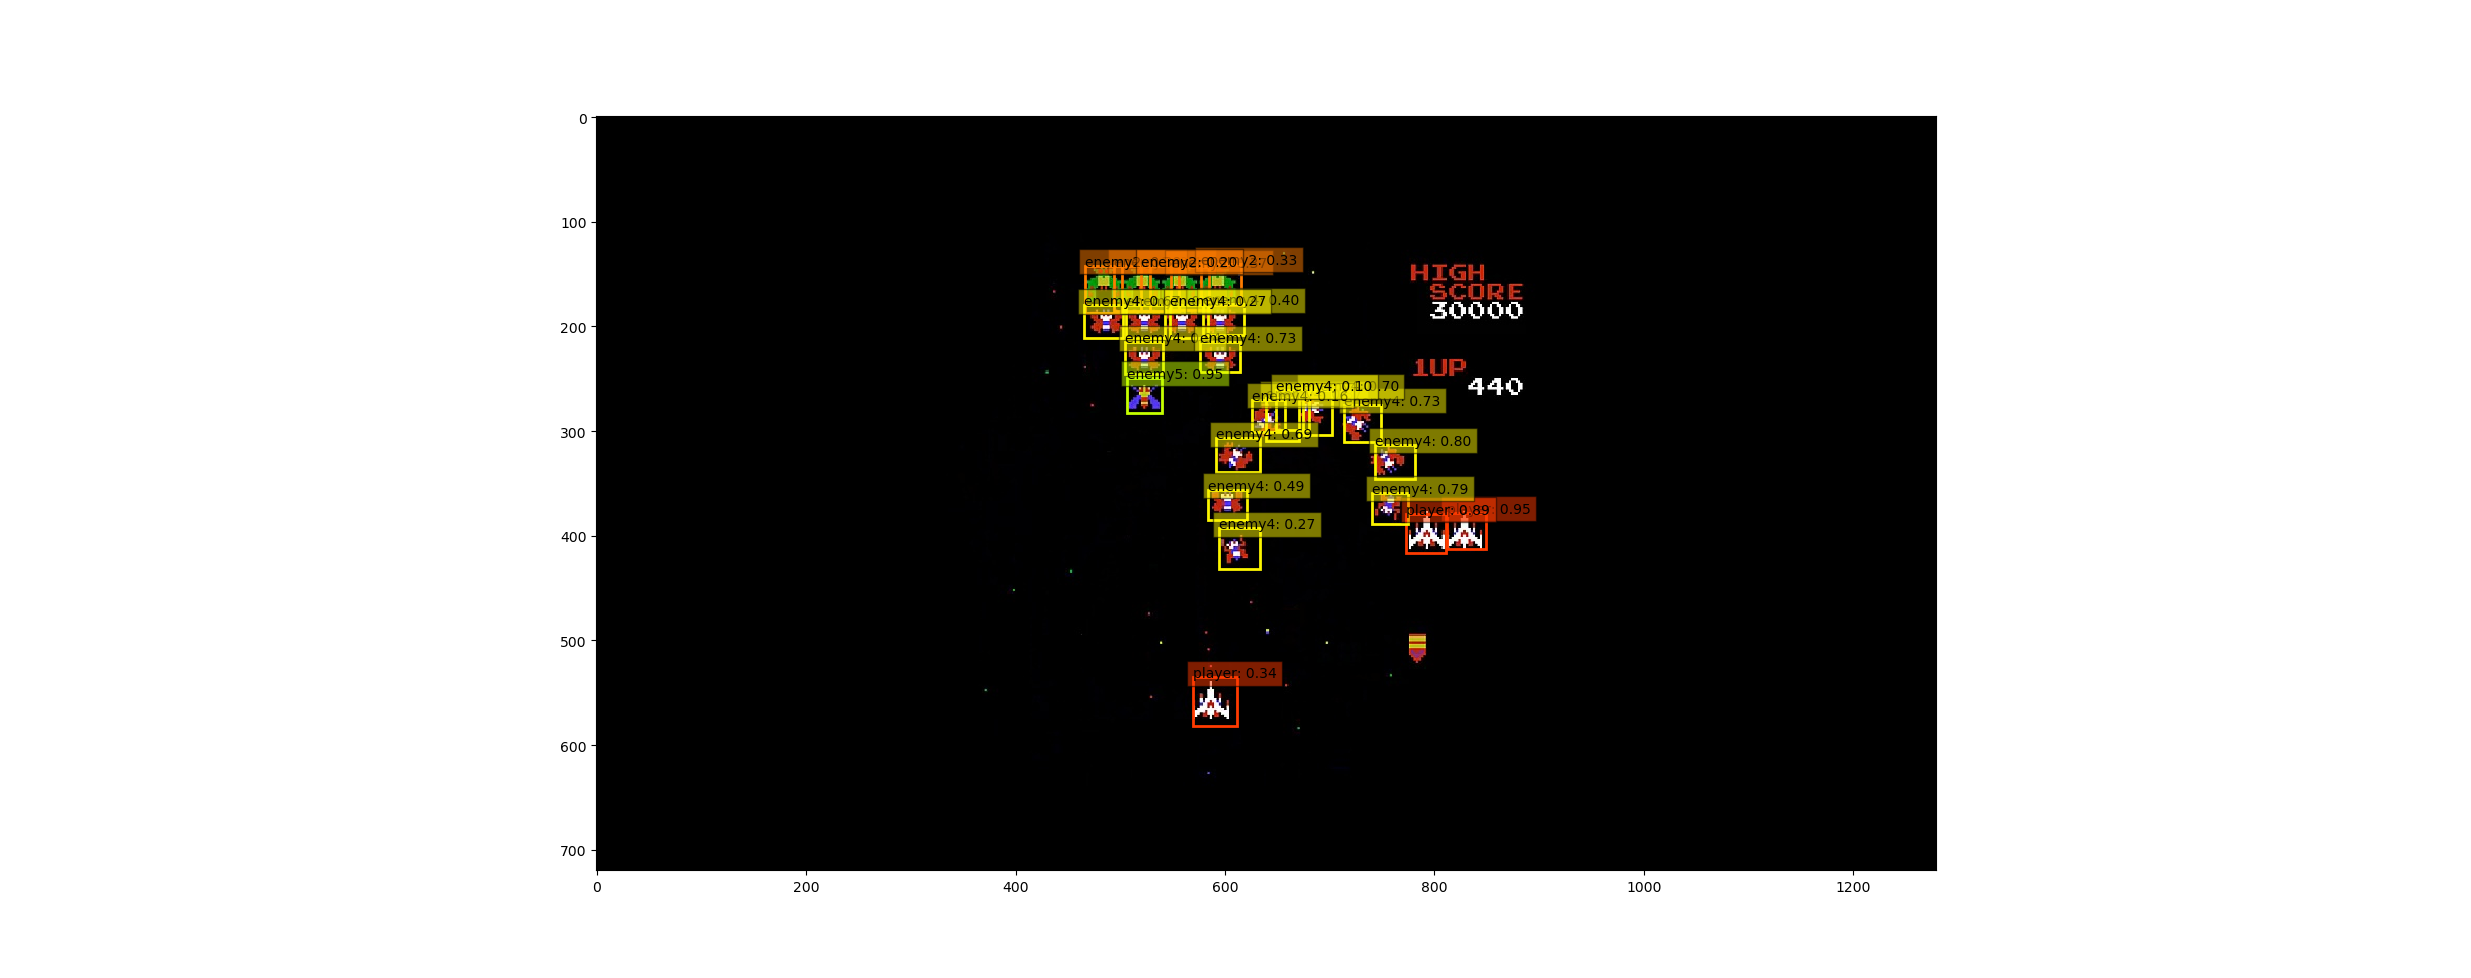
\includegraphics[width=\paperwidth]{d1.eps}}
\end{center}
\subsection{Detection Layer Result Sample 2}
\begin{center}
  \makebox[\textwidth]{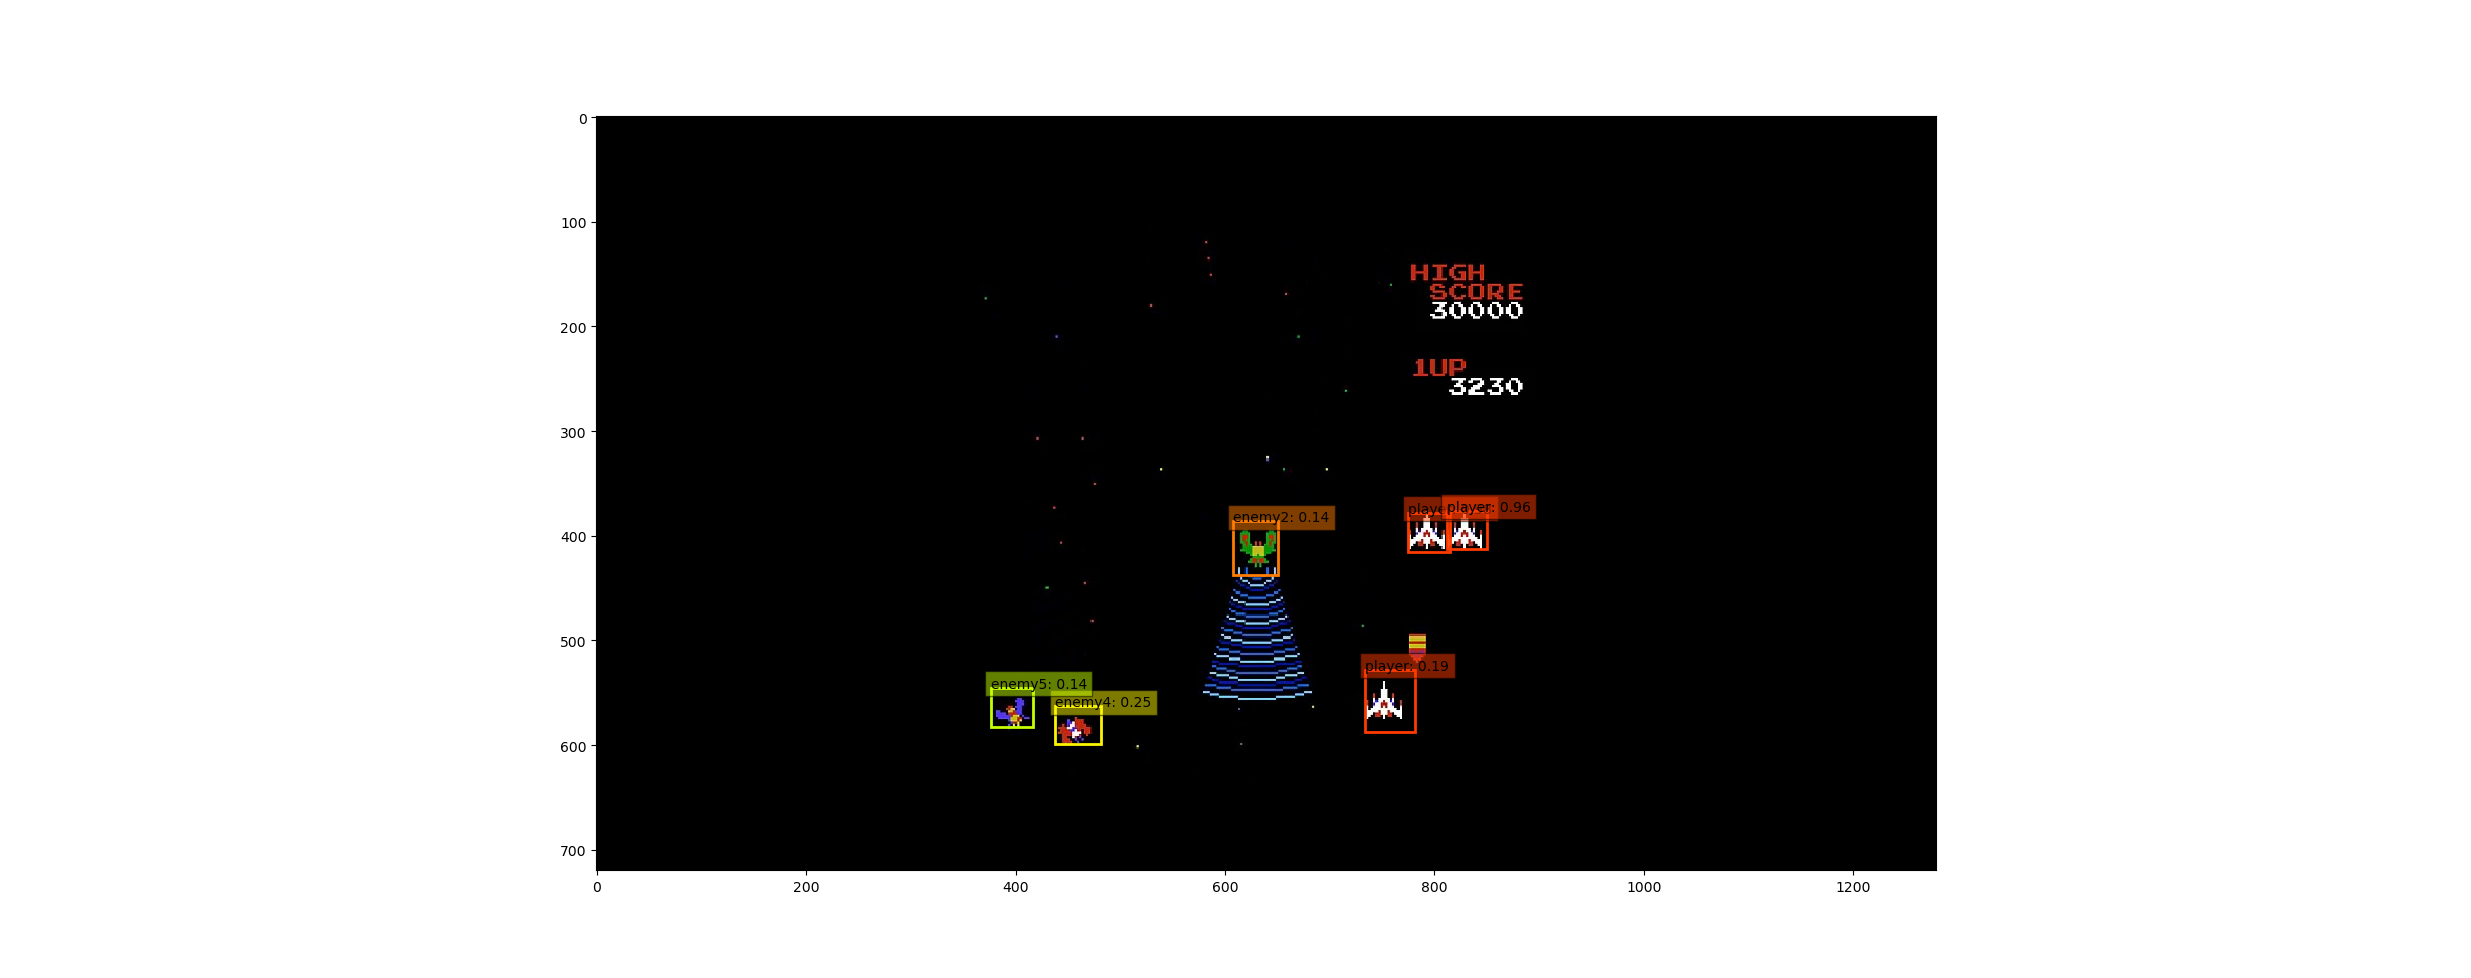
\includegraphics[width=\paperwidth]{d2.eps}}
\end{center}
\subsection{Training plot Loss v.s Accuracy}
\begin{center}
  \makebox[\textwidth]{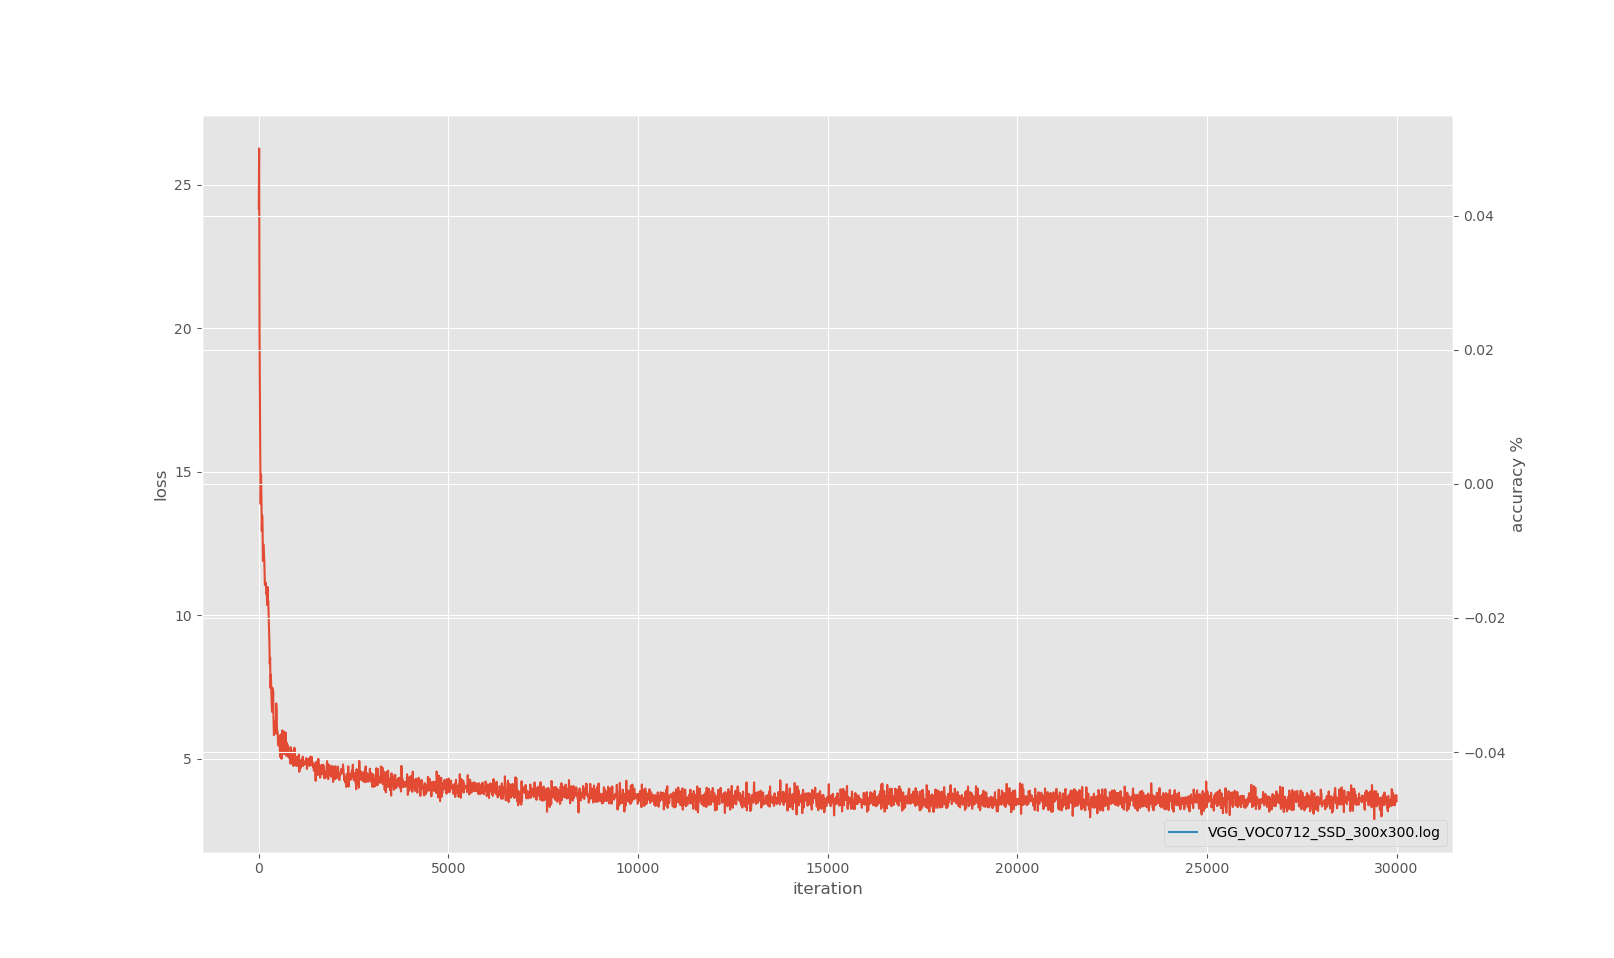
\includegraphics[width=\paperwidth]{plot.eps}}
\end{center}
\subsection{Final Project Setup}
\begin{center}
  \makebox[\textwidth]{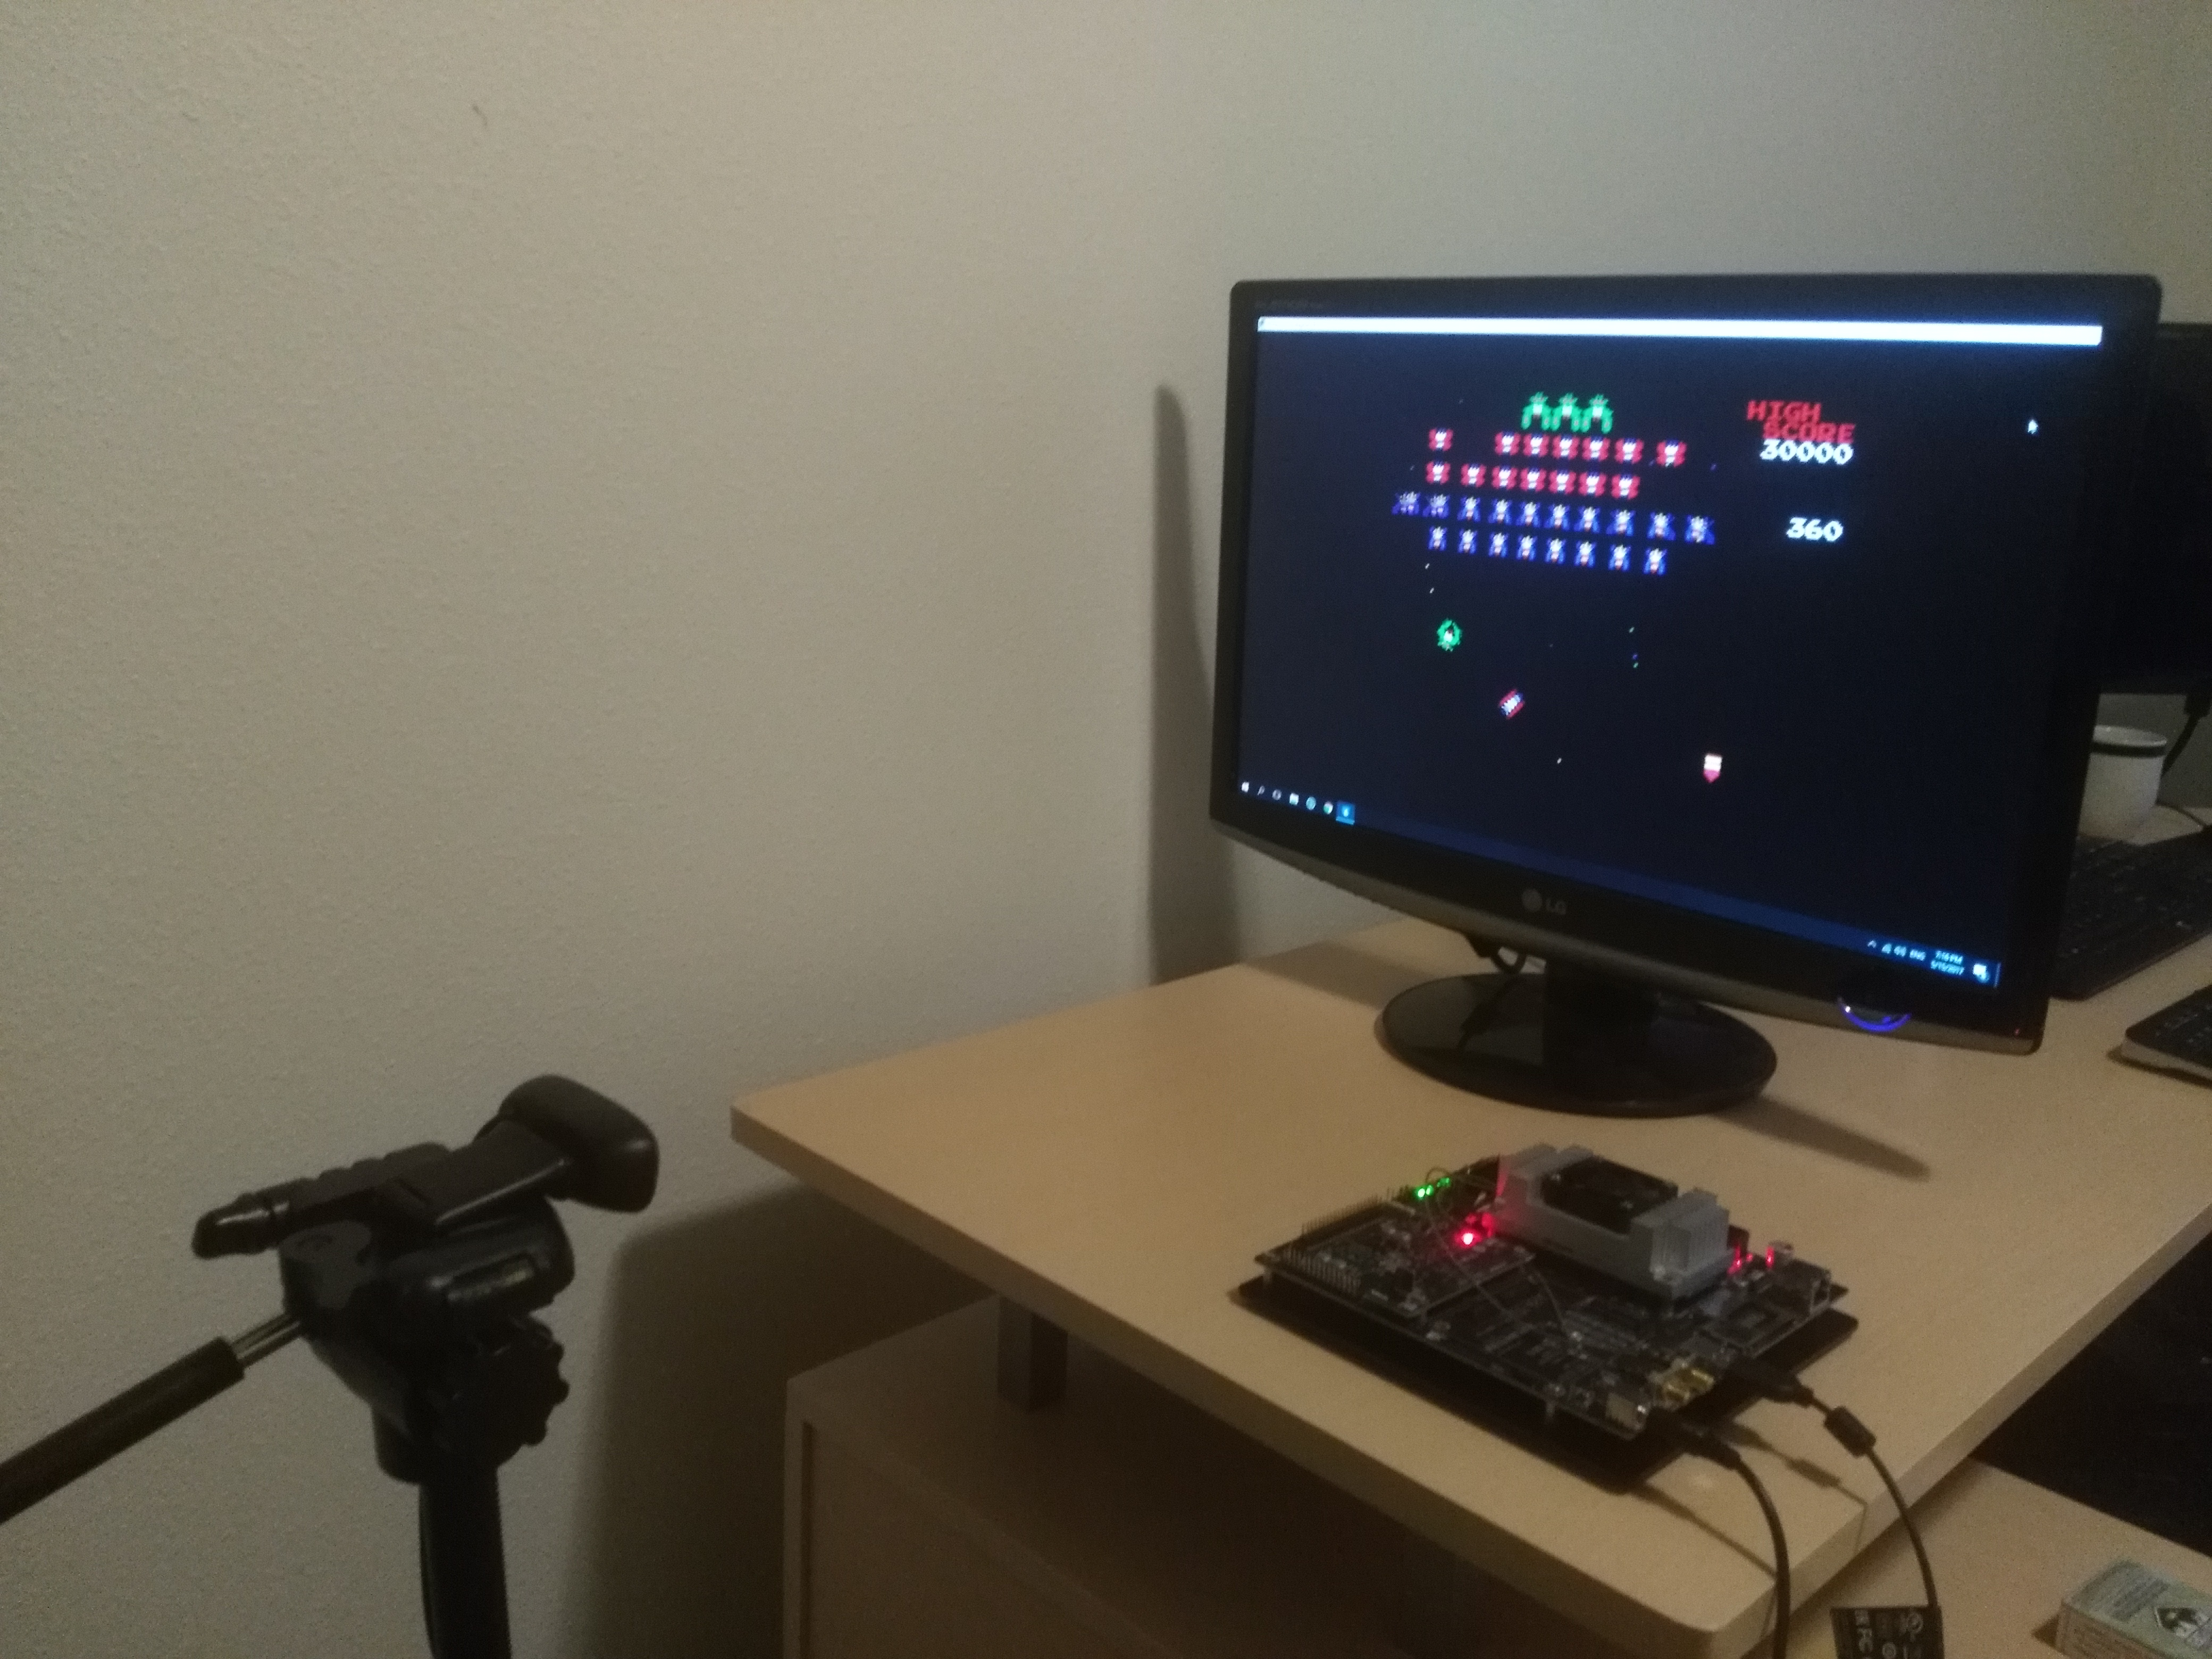
\includegraphics[width=\paperwidth]{setup.eps}}
\end{center}
\end{document}
